\section{概要}

\index{Collision}
Collisionモジュールは物理計算の基礎となる衝突判定機能を提供します.
\KLUDGE 事実上CollisionモジュールはPhysicsモジュールのサブモジュールとなっており,両者は密接に依存しています.
\KLUDGE ユーザは主として剛体に衝突判定用形状を割り当てる際にCollisionモジュールの機能を利用することになります.

\begin{figure}[t]
\begin{center}
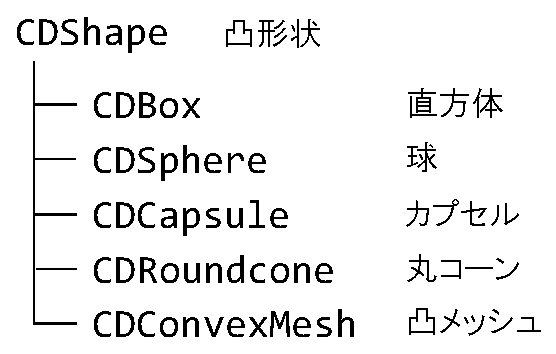
\includegraphics[width=.4\hsize]{fig/cdclass.eps}
\end{center}
\caption{Class hierarchy of Collision module}
\label{fig_cdclass}
\end{figure}

\index{CDShape}
Collisionモジュールのクラス階層をFig.\,\ref{fig_cdclass}に示します.
\KLUDGE 衝突判定形状はすべて\url{CDShape}から派生します.
\KLUDGE アルゴリズムの性質上,形状はすべて凸形状でなければなりません.

\section{形状の作成}

\KLUDGE 衝突判定形状は次の手順で作成・登録します.
\begin{enumerate}
\item 形状を作成する
\item 剛体へ形状を追加する
\item 形状の位置を設定する
\end{enumerate}
\KLUDGE 以下に順を追って説明します.

\KLUDGE まず形状を作成するには次のようにします.
\begin{sourcecode}
// given PHSdkIf* phSdk

CDBoxDesc desc;
desc.boxsize = Vec3d(1.0, 1.0, 1.0);

CDBoxIf* box = phSdk->CreateShape(desc)->Cast();
\end{sourcecode}
\KLUDGE 衝突判定形状のオブジェクトはPhysicsモジュールが管理します.
\KLUDGE このため,形状を作成するには\url{PHSdk}クラスの\url{CreateShape}関数を使います.
\url{PHSdk}については\ref{chap_physics}章を参照してください.
\KLUDGE 形状を作成するには,まず種類に応じたディスクリプタを作成し,寸法などのパラメータを設定します.
\KLUDGE この例では直方体クラス\url{CDBox}のディスクリプタを作成して一辺が$1.0$の立方体を作成します.
\KLUDGE ディスクリプタを指定して\url{CreateShape}を呼び出すと,対応する種類の形状が作成され,
\KLUDGE そのインタフェースが返されます.
\KLUDGE ただし戻り値は形状の基底クラスである\url{CDShape}のインタフェースですので,派生クラス(ここでは\url{CDBox})のインタフェースを得るには
\KLUDGE 上のように\url{Cast}関数で動的キャストする必要があります.

\KLUDGE 形状を作成したら,次にその形状を与えたい剛体に登録します.
\begin{sourcecode}
// given PHSolidIf* solid

solid->AddShape(box);         // first box
\end{sourcecode}
\KLUDGE 剛体クラス\url{PHSolid}については\ref{chap_physics}章を参照してください.
\KLUDGE ここで重要なことは,一度作成した形状は1つの剛体にいくつでも登録でき,また異なる複数の剛体にも登録できるということです.
\KLUDGE つまり,同じ形状を複数の剛体間で共有することで,形状の作成コストやメモリ消費を抑えることができます.

\url{AddShape}関数で登録した直後の形状は,剛体のローカル座標系の原点に位置しています.
\KLUDGE これを変更したい場合は\url{SetShapePose}関数を使います.
\begin{sourcecode}
solid->AddShape(box);         // second box
solid->AddShape(box);         // third box 

// move first shape 1.0 in x-direction
solid->SetShapePose(0, Posed(Vec3d(1.0, 0.0, 0.0), Quaterniond());

// rotate second shape 30 degrees along y-axis
solid->SetShapePose(1, Posed(Vec3d(),
                    Quaterniond::Rot(Rad(30.0), 'y')));
\end{sourcecode}
\url{SetShapePose}の第1引数は操作する形状の番号です.最初に\url{AddShape}した形状の番号が$0$で,\url{AddShape}するたびに$1$増加します.
\KLUDGE 形状の位置や向きは剛体のローカル座標系で指定します.
\KLUDGE また,形状の位置・向きを取得するには\url{GetShapePose}関数を使います.

\KLUDGE 以下ではSpringheadでサポートされている形状を種類別に解説します.

\subsection*{直方体}

\begin{figure}[t]
\begin{center}
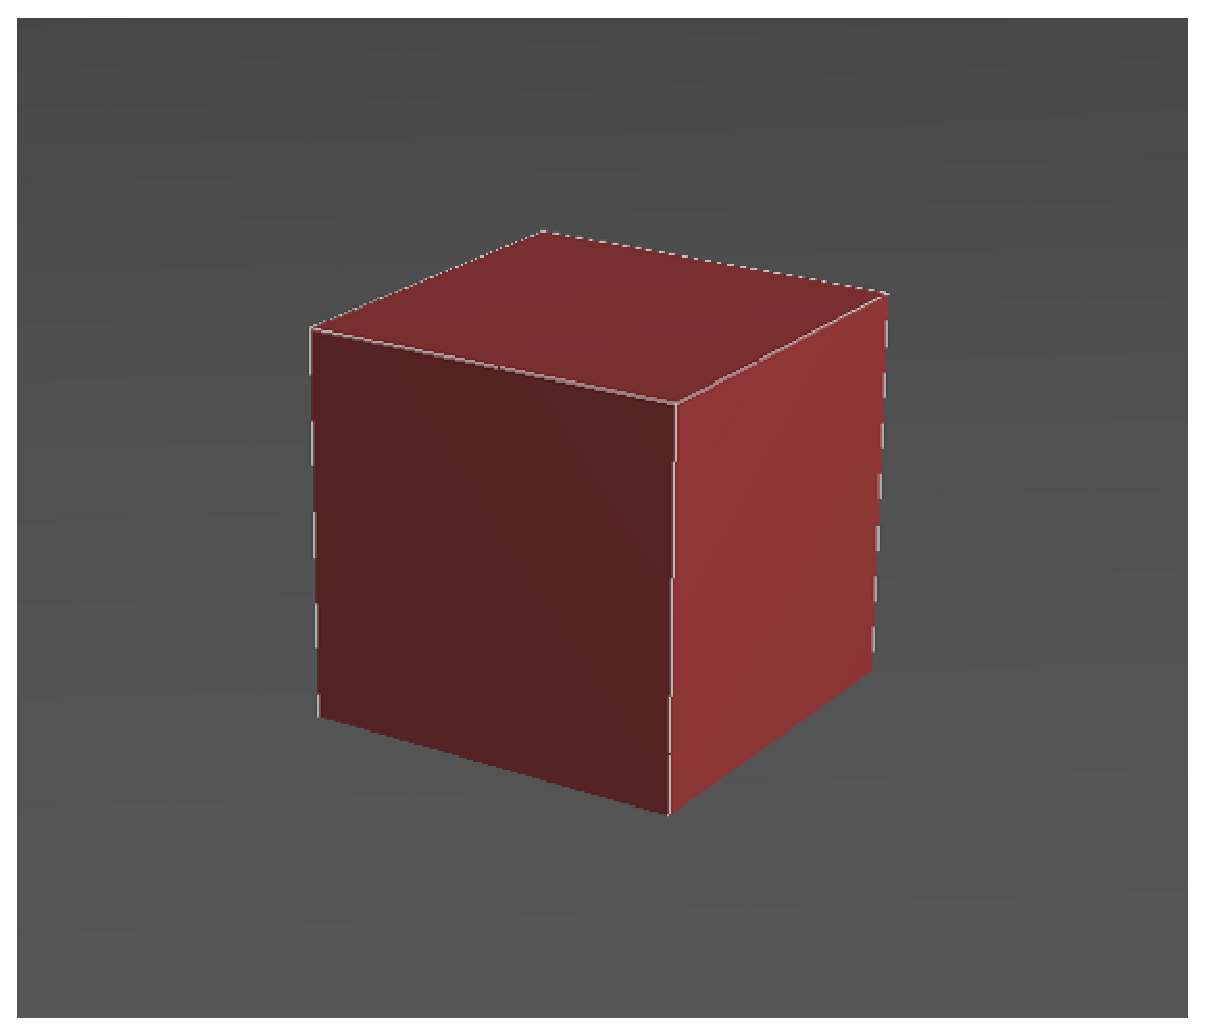
\includegraphics[width=.4\hsize]{fig/cdbox.eps}
\end{center}
\caption{Box geometry}
\label{fig_cdbox}
\end{figure}

\index{CDBox}
\index{ちょくほうたい@直方体}
\KLUDGE 直方体(Fig.\,\ref{fig_cdbox})のクラスは\texttt{CDBox}です.

\begin{center}
\begin{tabular}{lll}
\multicolumn{3}{l}{\texttt{CDBoxDesc}}					\\ \midrule
\texttt{Vec3f}	&	\texttt{boxsize}	& 各辺の長さ 	\\
\\
\multicolumn{3}{l}{\texttt{CDBoxIf}}					\\ \midrule
\multicolumn{2}{l}{\texttt{Vec3f GetBoxSize()}}			\\
\multicolumn{2}{l}{\texttt{void SetBoxSize(Vec3f)}}		\\
\end{tabular}
\end{center}


\subsection*{球}

\begin{figure}[t]
\begin{center}
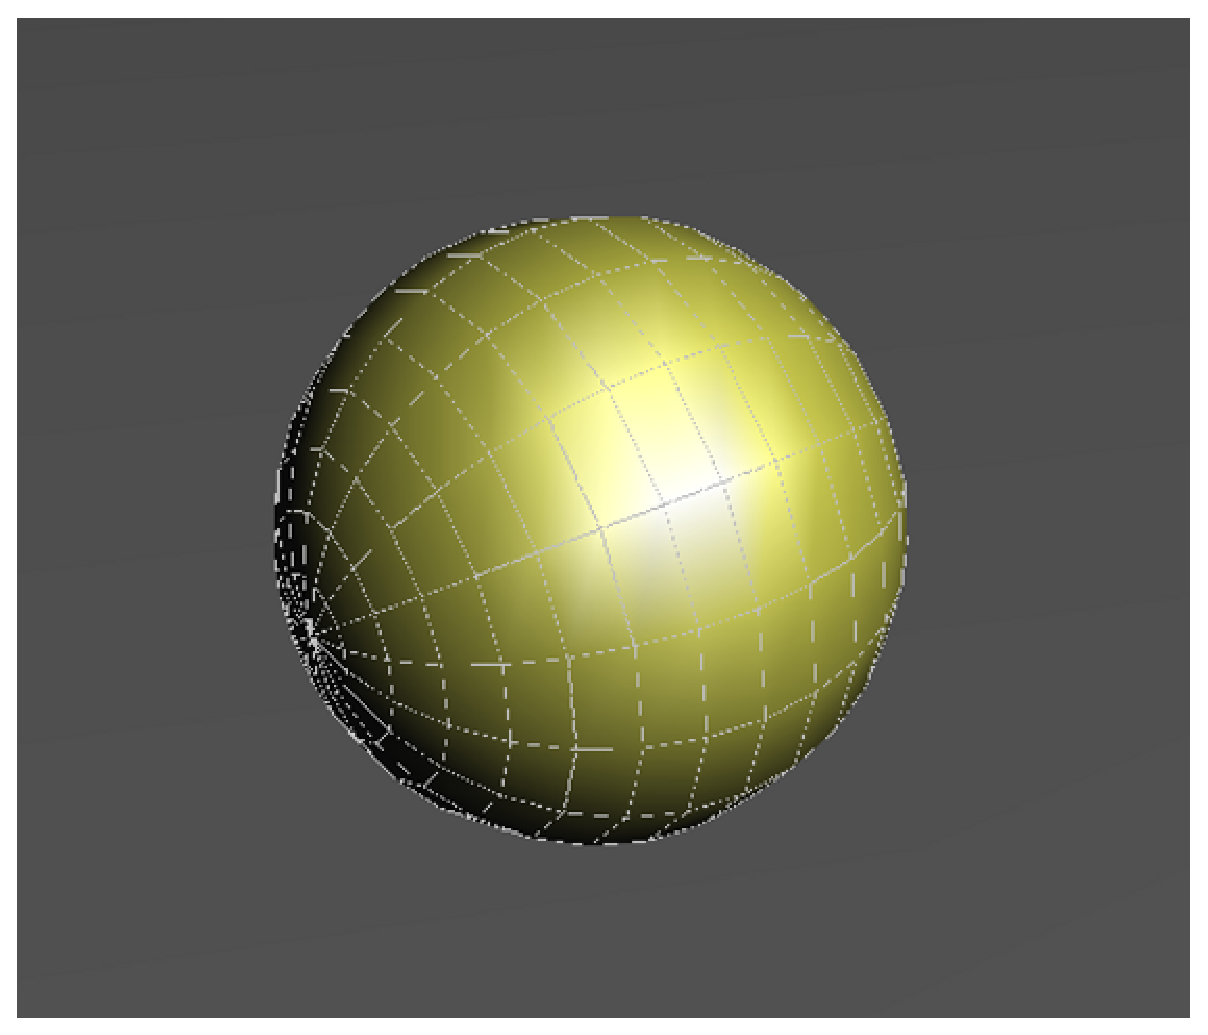
\includegraphics[width=.4\hsize]{fig/cdsphere.eps}
\end{center}
\caption{Sphere geometry}
\label{fig_cdsphere}
\end{figure}

\index{CDSphere}
\index{きゅう@球}
\KLUDGE 球(Fig.\,\ref{fig_cdsphere})のクラスは\url{CDSphere}です.

\begin{center}
\begin{tabular}{lll}
\multicolumn{3}{l}{\texttt{CDSphereDesc}}				\\ \midrule
\texttt{float}	&	\texttt{radius}	& 半径 				\\
\\
\multicolumn{3}{l}{\texttt{CDSphereIf}}					\\ \midrule
\multicolumn{2}{l}{\texttt{float GetRadius()}}			\\
\multicolumn{2}{l}{\texttt{void SetRadius(float)}}		\\
\end{tabular}
\end{center}


\subsection*{カプセル}

\begin{figure}[t]
\begin{center}
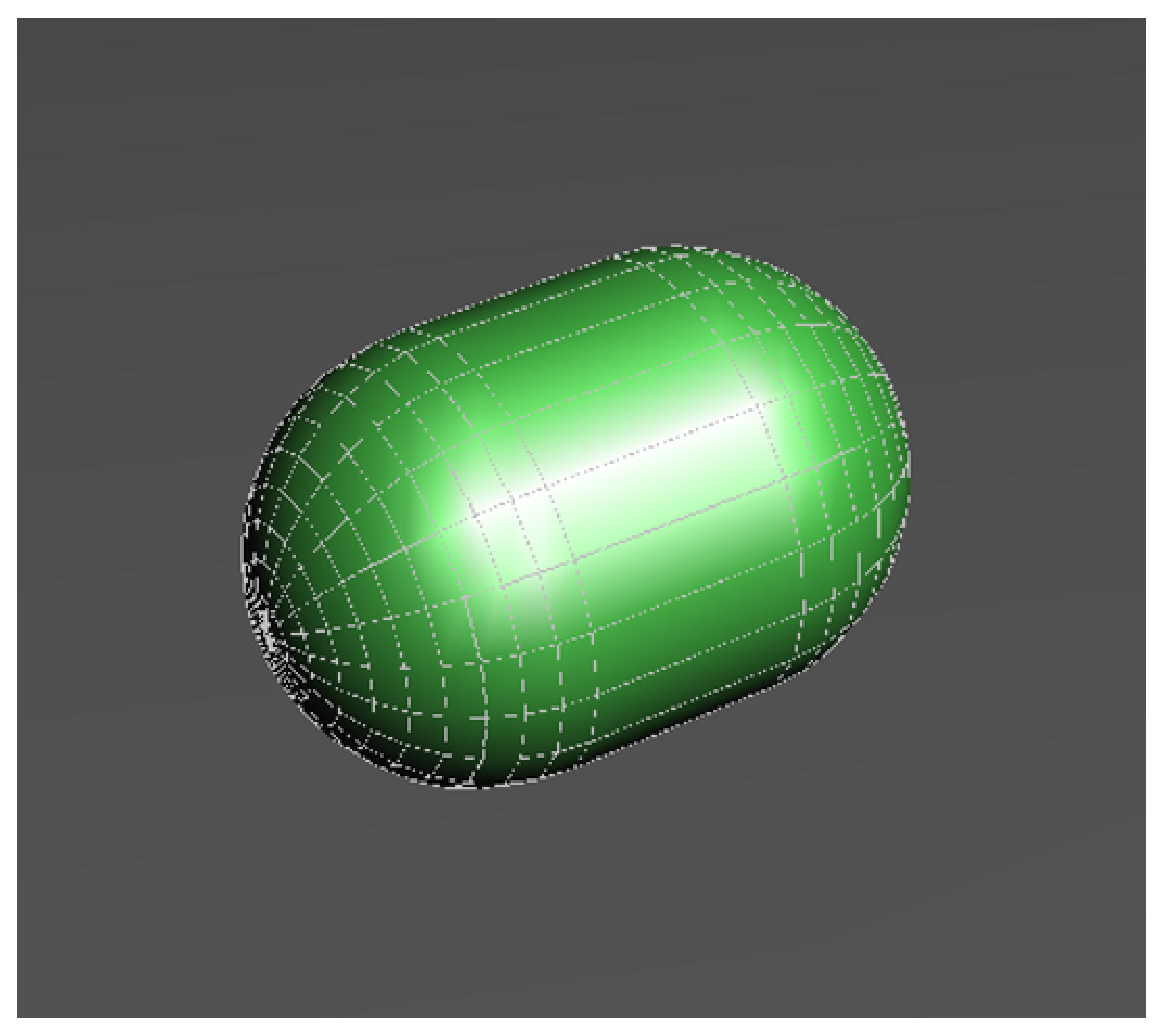
\includegraphics[width=.4\hsize]{fig/cdcapsule.eps}
\end{center}
\caption{Capsule geometry}
\label{fig_cdcapsule}
\end{figure}

\index{CDCapsule}
\index{かぷせる@カプセル}
\KLUDGE カプセル(Fig.\,\ref{fig_cdcapsule})のクラスは\url{CDCapsule}です.
\KLUDGE カプセルは円柱の両端に半球がついた形をしています.

\begin{center}
\begin{tabular}{lll}
\multicolumn{3}{l}{\texttt{CDCapsuleDesc}}				\\ \midrule
\texttt{float}	&	\texttt{radius}	& 半球の半径 		\\
\texttt{float}	&	\texttt{length} & 円柱の長さ		\\
\\
\multicolumn{3}{l}{\texttt{CDCapsuleIf}}				\\ \midrule
\multicolumn{2}{l}{\texttt{float GetRadius()}}			\\
\multicolumn{2}{l}{\texttt{void SetRadius(float)}}		\\
\multicolumn{2}{l}{\texttt{float GetLength()}}			\\
\multicolumn{2}{l}{\texttt{void SetLength(float)}}		\\
\end{tabular}
\end{center}


\subsection*{丸コーン}

\begin{figure}[t]
\begin{center}
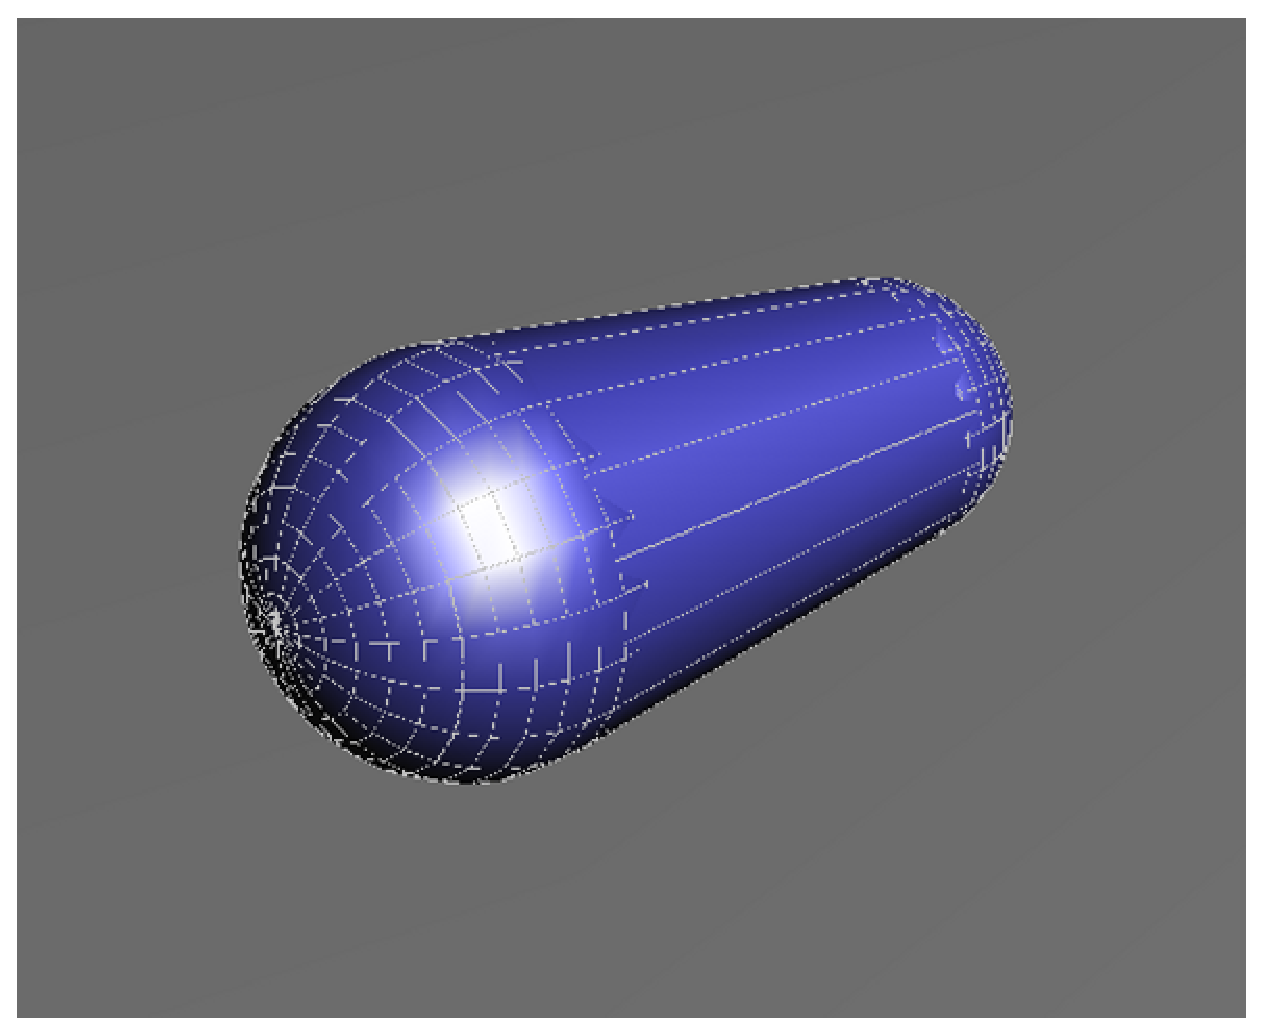
\includegraphics[width=.4\hsize]{fig/cdroundcone.eps}
\end{center}
\caption{Round cone geometry}
\label{fig_cdroundcone}
\end{figure}

\index{CDRoundCone}
\index{まるこーん@丸コーン}
\KLUDGE 丸コーン(Fig.\,\ref{fig_cdroundcone})のクラスは\url{CDRoundCone}です.
\KLUDGE 丸コーンはカプセルの両端の半径が非対称になったものです.

\begin{center}
\begin{tabular}{lll}
\multicolumn{3}{l}{\texttt{CDRoundConeDesc}}			\\ \midrule
\texttt{Vec2f}	&	\texttt{radius}	& 各半球の半径		\\
\texttt{float}	&	\texttt{length} & 半球間の距離		\\
\\
\multicolumn{3}{l}{\texttt{CDRoundConeIf}}				\\ \midrule
\multicolumn{2}{l}{\texttt{Vec2f GetRadius()}}			\\
\multicolumn{2}{l}{\texttt{void SetRadius(Vec2f)}}		\\
\multicolumn{2}{l}{\texttt{float GetLength()}}			\\
\multicolumn{2}{l}{\texttt{void SetLength(float)}}		\\
\multicolumn{2}{l}{\texttt{void SetWidth(Vec2f)}}		\\
\end{tabular}
\end{center}

\texttt{SetWidth}関数は,丸コーンの全長を保存したまま半径を変更します.


\subsection*{凸メッシュ}

\begin{figure}[t]
\begin{center}
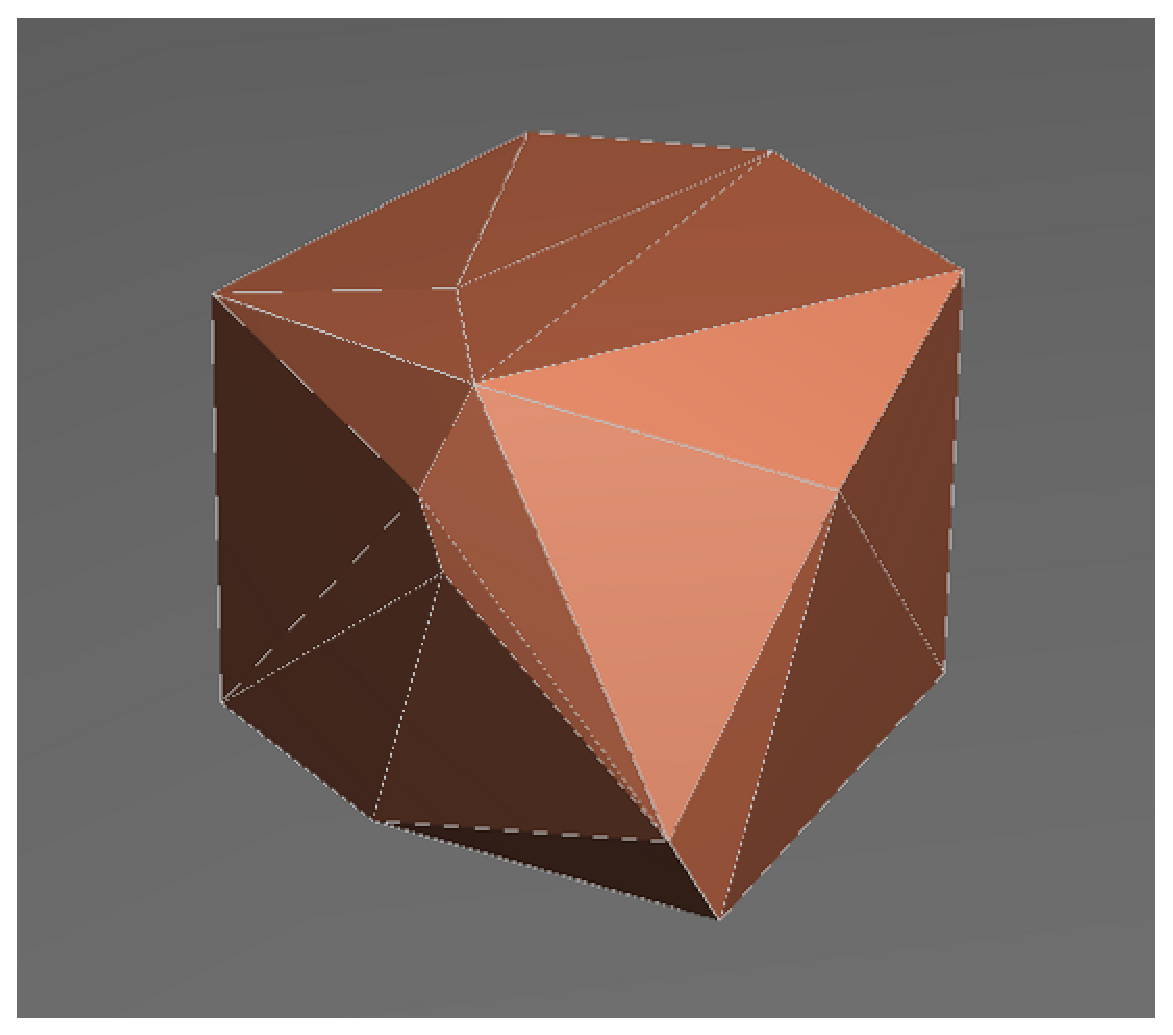
\includegraphics[width=.4\hsize]{fig/cdconvexmesh.eps}
\end{center}
\caption{Convex mesh geometry}
\label{fig_cdconvexmesh}
\end{figure}

\index{CDConvexMesh}
\index{とつめっしゅ@凸メッシュ}
\KLUDGE 凸メッシュ(Fig.\,\ref{fig_cdconvexmesh})のクラスは\url{CDConvexMesh}です.
\KLUDGE 凸メッシュとは凹みや穴を持たない多面体です.
\KLUDGE 頂点座標を指定することで自由な形を作成することができます.

\begin{center}
\begin{tabular}{lll}
\multicolumn{3}{l}{\texttt{CDConvexMeshDesc}}						\\ \midrule
\texttt{vector<Vec3f>}	&	\texttt{vertices}	& 頂点座標の配列	\\
\\
\multicolumn{3}{l}{\texttt{CDConvexMeshIf}}					\\ \midrule
\multicolumn{2}{l}{\texttt{Vec3f* GetVertices()}}			& 頂点配列の先頭アドレス	\\
\multicolumn{2}{l}{\texttt{int NVertex()}}					& 頂点数					\\
\multicolumn{2}{l}{\texttt{CDFaceIf* GetFace(int i)}}		& $i$番目の面				\\
\multicolumn{2}{l}{\texttt{int NFace()}}					& 面数						\\
\end{tabular}
\end{center}

\KLUDGE 凸メッシュが作成される際,\texttt{CDConvexMeshDesc::vertices}に格納された頂点を内包する最小の凸多面体(凸包)が作成されます.
\KLUDGE 多面体の面を表す\texttt{CDFace}のインタフェースを以下に示します.

\begin{center}
\begin{tabular}{lll}
\multicolumn{3}{l}{\texttt{CDFaceIf}}						\\ \midrule
\multicolumn{2}{l}{\texttt{int* GetIndices()}}				& 頂点インデックス配列の先頭アドレス	\\
\multicolumn{2}{l}{\texttt{int NIndex()}}					& 面の頂点数							\\
\end{tabular}
\end{center}

\texttt{NIndex}は面を構成する頂点の数を返します(通常$3$か$4$です).
\KLUDGE 面は頂点配列を直接保有せず,インデックス配列として間接的に頂点を参照します.
\KLUDGE したがって,面の頂点座標を得るには
\begin{sourcecode}
// given CDConvexMeshIf* mesh
CDFaceIf* face = mesh->GetFace(0);        // get 0-th face
int* idx = face->GetIndices();
Vec3f v = mesh->GetVertices()[idx[0]];    // get 0-th vertex
\end{sourcecode}
\KLUDGE とします.

\section{物性の指定}
\label{sec_collision_material}

\index{PHMaterial}
\index{ぶっせい@物性}
\KLUDGE 形状には摩擦係数や跳ね返り係数などの物性を指定することができます.
\KLUDGE 形状の基本クラスである\texttt{CDShape}のディスクリプタ\texttt{CDShapeDesc}は\texttt{PHMaterial}型の変数\texttt{material}を持っています.

\begin{center}
\begin{tabular}{lll}
\multicolumn{3}{l}{\texttt{PHMaterial}}							\\ \midrule
\texttt{float}	&	\texttt{density}		& 密度				\\
\texttt{float}	&	\texttt{mu0}			& 静止摩擦係数		\\
\texttt{float}	&	\texttt{mu}				& 動摩擦係数		\\
\texttt{float}	&	\texttt{e}				& 跳ね返り係数		\\
\texttt{float}	&	\texttt{reflexSpring}	& 跳ね返りバネ係数(ペナルティ法)	\\
\texttt{float}	&	\texttt{reflexDamper}	& 跳ね返りダンパ係数(ペナルティ法)\\
\texttt{float}	&	\texttt{frictionSpring}	& 摩擦バネ係数(ペナルティ法)	\\
\texttt{float}	&	\texttt{frictionDamper}	& 摩擦ダンパ係数(ペナルティ法)\\
\end{tabular}
\end{center}

\KLUDGE 形状作成後に物性を指定するには\texttt{CDShapeIf}の関数を使います.

\begin{center}
\begin{tabular}{lll}
\multicolumn{3}{l}{\texttt{CDShapeIf}}						\\ \midrule
\multicolumn{2}{l}{\texttt{void SetDensity(float)}}				& \\
\multicolumn{2}{l}{\texttt{float GetDensity()}}					& \\
\multicolumn{2}{l}{\texttt{void SetStaticFriction(float)}}		& \\
\multicolumn{2}{l}{\texttt{float GetStaticFriction()}}			& \\
\multicolumn{2}{l}{\texttt{void SetDynamicFriction(float)}}		& \\
\multicolumn{2}{l}{\texttt{float GetDynamicFriction()}}			& \\
\multicolumn{2}{l}{\texttt{void SetElasticity(float)}}			& \\
\multicolumn{2}{l}{\texttt{float GetElasticity()}}				& \\
\multicolumn{2}{l}{\texttt{void SetReflexSpring(float)}}		& \\
\multicolumn{2}{l}{\texttt{float GetReflexSpring()}}			& \\
\multicolumn{2}{l}{\texttt{void SetReflexDamper(float)}}		& \\
\multicolumn{2}{l}{\texttt{float GetReflexDamper()}}			& \\
\multicolumn{2}{l}{\texttt{void SetFrictionSpring(float)}}		& \\
\multicolumn{2}{l}{\texttt{float GetFrictionSpring()}}			& \\
\multicolumn{2}{l}{\texttt{void SetFrictionDamper(float)}}		& \\
\multicolumn{2}{l}{\texttt{float GetFrictionDamper()}}			& \\
\end{tabular}
\end{center}

\KLUDGE 物性に基づいた接触力の具体的な計算法については第\ref{sec_physics_contact}節を参照して下さい.

\section{幾何情報の計算}

\KLUDGE 形状に関する幾何情報を計算する関数を紹介します.

\begin{center}
\begin{tabular}{lll}
\multicolumn{3}{l}{\texttt{CDShapeIf}}							\\ \midrule
\multicolumn{2}{l}{\texttt{float CalcVolume()}}					& 体積を計算		\\
\multicolumn{2}{l}{\texttt{Vec3f CalcCenterOfMass()}}			& 質量中心を計算	\\
\multicolumn{2}{l}{\texttt{Matrix3f CalcMomentOfInertia()}}		& 慣性行列を計算	\\
\end{tabular}
\end{center}

\texttt{CalcVolume}は形状の体積を計算します.体積に密度(\texttt{GetDensity}で取得)を掛ければ質量が得られます.
\texttt{CalcCenterOfMass}関数は,形状のローカル座標系で表された質量中心の座標を計算します.
\texttt{CalcMomentOfInertia}関数は,形状のローカル座標系で表された質量中心に関する慣性行列を計算します.
\KLUDGE ただし,密度を$1$とした場合の値が返されますので,実際の慣性行列を得るには密度を掛ける必要があります.

